\documentclass{article}
\usepackage[utf8]{inputenc}
\usepackage{amsmath}   
\usepackage{mathtools}
\usepackage{graphicx}
\usepackage{subcaption}
\usepackage{float}
\usepackage{hyperref}
\usepackage{listings}
\usepackage[labelfont=bf]{caption}
\usepackage[margin=3.75cm]{geometry}

%\usepackage{qtree}
%\usepackage{tikz}
%\usepackage{tikz-qtree}

%\usepackage[]{algorithm2e}
\hyphenation{ECMAScript JavaScript escodegen esprima}

\lstset{
	basicstyle=\footnotesize\ttfamily,
}

\title{
Probabilistic Programming
%\\\vspace{4 mm}\underline{\Large House Lannister}
}

\author{
	Carlos Diaz, Dan Hassin, Charles Lehner, Dan Viterise \\
    \vspace{0pt}\\ Department of Computer Science \\University of Rochester
}

\date{April 21, 2014}

\begin{document}

\maketitle

\begin{abstract}
	We present Probabilistic Programming, a system for generating JavaScript programs and code snippets based off a corpus of JavaScript source files.
	In this paper, we will demonstrate storing statistical
    data from non-linear structures (abstract syntax trees of programs) in a Markov model,
    and of course using the model to generate new trees. We present a proof of concept for a web-based
    assistive program editor that utilizes this technology to guide programmers through
	constructing JavaScript programs.
\end{abstract}

\section{Introduction}

This paper will begin by discussing Markov chains and how we set out to use them for our goal. We will then describe in detail how we implemented a Markov chain for program syntax trees, how we were able to generate code using it, and finally we'll discuss our results and address the limitations of our product.

\subsection{Markov chain}

A Markov chain is a mathematical system that undergoes a stochastic process whereby
the current state and a set of probabilities are used to determine what state
to transition to next. In the most simple case of a Markov chain, the next action is based
only upon the current state and all other previous actions are forgotten.
Thus, this process is essentially ``memoryless'' because all past states can be
forgotten once a new state is reached \cite{markov}. In this way, Markov chains can be likened
to deterministic finite automata. So while they cannot remember a limitless amount of their history,
calling them ``memoryless'' may be misleading, as they can indeed be implemented to remember a fixed
size of their state history.

Markov chains find application in many different fields. Familiar with Markov chains used for generating random human-sounding text (by training a model based on bigrams and trigrams of common speech), we were interested in perhaps more novel domains. We chose to use a Markov chain to drive code generation, because, like text, we feel that code can be personal and expressive, and the idea of generating code possibilities from a training set seemed like exciting research. It was also challenging -- since randomly generating code tokens would most likely produce syntactically invalid programs, we looked at program abstract syntax trees. And as the research developed, we found ourselves with a new vision of a semifeasable product.

\subsection{Emerging goal}

For many novice programmers, programming can seem like a confusing and
tedious activity. It can be unclear for many new programmers where they should
begin and what should come next while coding. They may conceptually understand
what the next step should be, and yet be unable to express it with code. Or, they
could be unsure of the right next step conceptually, and some code could inspire
them to understand it.

Even once one becomes more
adept at programming, he or she may notice typing the same or
similar lines of code in each new program. This repetitiveness slows down
the user and can make programming more tiresome a task.

The prospect of using a Markov chain to generate code snippets in an assistive, predictive, integrated development environment (IDE) for JavaScript seemed to be a natural progression from our research. Our final product, a Probabilistic Programming
web application, allows a user to code in JavaScript by way of selecting from
a list of suggestions for the user's next line of code. We imagine that this won't only be helpful for new programmers,
but that this system would allow for expert programmers to write code with more ease and efficiency.

% overview of markov chain

\section{Tree-based Markov chain}

\subsection{Abstract syntax trees}

An abstract syntax tree (AST) is a tree-based, rather than text-based, representation of a program.
Such a tree is generated using the grammar rules of a programming language and text input. In the tree, \emph{nodes}
are language control structures such as {\tt for} loops, {\tt if} statements, variable and function
declarations, and so on. The \emph{edges} connecting a parent node to its children represent the different \emph{features}
of that node. For instance, a {\tt for} loop would have the features \emph{init} (e.g. {\tt var i = 0;}),
\emph{test} (e.g. {\tt i < array.length;}), \emph{update} (e.g. {\tt i++}), and a \emph{body} (a list
of statements that should be executed per loop iteration). To implement lists, we include the additional
\emph{follow} edge as a feature to all statements, which would connect a statement node to the next statement
in the list. If the statement is last in its container list, we connect its \emph{follow} edge to a special
{\tt {\_end}} node. (See figure~\ref{fig:sample-ast} for an example of a AST.)

% \begin{center}

% \begin{tikzpicture}[level distance=1.5cm,
% level 1/.style={sibling distance=3.5cm},
% level 2/.style={sibling distance=1cm}]

% \node (Root) {Program}
% child {
%     node {for} edge from parent node[draw=none] {\emph{body}}
%     child { node {VD} edge from parent node[draw=none] {\emph{init}} }
% };

% \end{tikzpicture}

% \end{center}

Our system deals with programs at the level of AST's as they provide more structure and modularity than text.
We use the syntax tree format of Mozilla's Parser API \cite{parser api}, and \emph{esprima} \cite{esprima}, an ECMAScript
(the language standard of which JavaScript is an implementation)
parser, to transform program source code into an AST of this format.

\subsection{Our Markov chain}

To build our Markov chain structure, we parse a corpus of JavaScript files into their
respective AST's, and then collect statistics from these trees to establish probability distributions of nodes for a given AST context. 

An \emph{AST path} is a list of items, alternating between node types and features, that encodes the unique position of a 
specific node in the AST. The \emph{probability distribution} for an AST path is the set of possible node types or values that would appear in the
syntax tree following the given path, and the respective probabilities of their
occurrence at that point. The model maps AST paths to the probability distributions of node types (or values, as we'll see later) for that given
path. 

More formally, given a depth $d$ (indicating how many nodes we should backtrace) for a given
${node}_d$ and feature ${edge}_d$, the generation of ${node}_d$'s child node given by
 ${edge}_d$ can be expressed by the following function $f$: \begin{align*}
f({node}_1, {edge}_1, ..., {node}_{d}, {edge}_{d}) = \begin{dcases*}
		{newnode_1},	&	$P({newnode_1})$ \\
		{newnode_2},	&	$P({newnode_2})$ \\
		...\\
		{newnode_n},    &   $P({newnode_n})$ \\
	\end{dcases*},
\end{align*}

where \begin{align*}
\sum\limits_{i = 0}^n P({newnode_i}) = 1.
\end{align*}

\noindent and ${Path}({node}_1, {edge}_1) = {node}_2$, ${Path}({node}_2, {edge}_2) = {node}_3$, ..., ${Path}({node}_d, {edge}_d) = {newnode}_k$, where ${newnode}_k$ is randomly selected from ${newnode}_1, ..., {newnode}_n$ given the probabilities $P({newnode_1}), ..., P({newnode_n})$. From this it can be seen that generating programs is simply a repetitive application of this function, where for the chosen ${newnode}_k$, we can generate each child of ${newnode}_k$ with the following formula. \begin{align*} &\forall {edge} \in {Features}({newnode}_k), \\
& \hspace{3em} {Path}({newnode}_k, {edge}) = f({node}_2, {edge}_2, ..., {node}_{d}, {edge}_{d}, {newnode}_k, {edge}).
\end{align*}

This process will eventually terminate as the probability of generating {\tt \_end} nodes for a \emph{follow} edge will always be non-zero -- the programs we parse into our corpus are surely finite -- and such nodes have no features to be ``expanded.''

\subsection{Implementation}

\subsubsection{Data structure}

Building the Markov chain model means being able to provide the probability distribution of new nodes for arbitrary input,
as described by the function in Section 2.2. To do this, we construct a data structure using JavaScript Object Notation (JSON),
a structural format useful for ease of specification and integration with JavaScript programs.

The data structure is a hash table (also commonly called a map, dictionary, or associative array), that, on a given input, returns another hash table for paths that begin with that input. This behavior is repeated until the number of inputs reaches the desired depth, at which point a final hash table, mapping the node type to its probability distribution, is returned. This, in effect, is modularizing the function $f$ described above, so that we can reach the probability distribution with minimal code and data duplication. This is demonstrated by following example, given  ${depth} = 2$. \begin{align*}
lookup(lookup(lookup(lookup({Model}, {node}_1), {edge}_1), {node}_2), {edge}_2) = \textbf{P}({newnodes}).
\end{align*}

\subsubsection{Building the model}

We first obtain collection of JavaScript programs in AST form. We then run the following algorithm to construct our model:

\begin{verbatim}
procedure addToModel(node, path):
    model = CorpusModel
    for each elem in path[path.length-depth*2 .. path.length]:
        model = model[elem]
    model[node.type] += 1
    model[_total] += 1
    for each feature of node:
        temp_path = path + [node.type, feature]
        if node.feature is list of nodes:
            for each item in node.feature:
                addToModel(item, temp_path)
                temp_path += [item.type, "FOLLOW"]
            addToModel(END_NODE, temp_path)
        else:
            addToModel(node.feature, temp_path)

for each parsed AST:
    addToModel(AST.root, [])
\end{verbatim}

For each AST, we walk through every node in the tree by recursively exploring each feature\footnote{While we use \emph{follow} as if it were a feature edge, programs encoded in the AST's we parse use arrays of nodes (rather than linked-lists as we represent them) for a collection of statements. The given pseudocode demonstrates how we can transform an array into a linear sequence of edges.} of each node. In each call to explore a node's feature, we maintain the path up until that node by appending to it the node type and the name of the feature to reach the wanted child. We trim the beginning of the path off so that the length of the path is appropriate with respect to the chosen depth (i.e. so that $|path| = 2*d$).\footnote{Note that this requires that the path is at least of length $2*depth$. If the path is shorter than this, it represents not having at least $d$ levels of context. This can occur, say, for the first statement in the entire program, where there are no preceding nodes in its AST path. For these cases, we add the ``{\tt \_null}'' feature until we reach the desired depth (omitted in the pseudocode.)} We traverse through the layers of hash tables, creating the path elements if they don't already exist, add the node type to the probability distribution if it isn't already, and then increment a counter associated with that node type. We also increment a ``{\tt \_total}'' counter for the convenience of the generator program.

When this process is complete, the JSON object is saved to a file and can be augmented by more code samples thereafter. (An example of such a model is shown in figure~\ref{fig:sample-model} in the Appendix. In this model we see, for instance, that the path
[\emph{Program, body, VariableDeclaration, declarations}] leads to
\emph{VariableDeclarator} with probability 1. This indicates that a \emph{Program}
node whose \emph{body} is a \emph{VariableDeclaration} always has a declaration that is of
type \emph{VariableDeclarator}.)

\subsection{Generating code}

Code can be generated rather easily using the approach explained in Section 2.2. The program tree is built up one node at a time, each one generated based on its unique AST path. The following algorithm demonstrates this process.

\clearpage

\begin{verbatim}
procedure generateNode(model, path):
    for each elem in path[path.length-depth*2 .. path.length]:
        model = model[elem]
    nodeType = pickRandomNodeType(model)
    node = {`type':nodeType}
    for each feature of nodeType:
        new_path = path + [node.type, feature]
        if feature is a list feature:
            nodes = []
            while (newNode = generateNode(model, new_path) != END_NODE:
                nodes += [nodeNode]
                new_path += [newNode.type, "FOLLOW"]
            node.feature = nodes
        else:
            node.feature = generateNode(model, new_path)
    return node

generateNode(CorpusModel, [])
\end{verbatim}

The algorithm looks very similar to the parse algorithm, as it is almost the same process, simply inverted. Rather than examine nodes, determine a path by building it up, and then increment a count in the model, this algorithm first finds the counts in the model for a \emph{given} path, generates a node, and generates nodes for all of that node's features recursively. The result is a generated AST for our program, which is then fed into \emph{escodegen} \cite{escodegen}, an ECMAScript code generator to output program source code that we can display and run.

To generate random programs, we always begin with a ``Program'' node, and then add nodes to its \emph{body} feature (an array.) However, we quickly found that while entertaining, generating random programs had little potential for real application. Instead, we turned to generating code snippets (to be placed in specific contexts of the syntax tree.) Since our algorithm was general enough for this purpose, no more had to be done besides knowing the path for the node we wanted to generate.

\subsubsection{Identifiers and literals}

Naturally, identifiers and literals are a very large part of programming. Without them, code would be entirely unspecific, and would only consist of syntactic symbols and keywords. Yet they pose an issue with code generation, as we found generating identifiers or literals that are likely to be what the user is expecting an especially difficult problem to solve, let alone model. Struggling to come up with a simple, intelligent, and robust solution, and short on time, we fell back to using our existing Markov approach.

In the current implementation of this system, following the paths [\emph{Identifier}, \emph{Name}], or [\emph{Literal}, \emph{Raw}] result not in node types, but rather in the text of the identifier names or literal values. This way, generating identifiers and literals is simply a probabilistic process like the rest of the code generation. Of course, this means that sometimes identifiers are added that are not in scope, that have mismatched types, or that simply make no semantic sense. (But adjusting $depth$ did seem to make programs more meaningful, as expected. This can be seen experimentally by modifying depth on our web IDE, which is discussed in Section 4.1.)

%\lstinputlisting[caption=Scheduler, style=json]{../rand.js}

\section{Applications}

\subsection{\emph{vim} autocomplete script}

We integrated our model into the text editor vim to offer autocompletion
suggestions of programs upon the user's request, using vim's
\texttt{completefunc} feature. When the user is editing a JavaScript file in vim with
this feature, they may press a keyboard command to get a list of program
snippets to choose from. The snippets are generated in the context of the
program path at cursor's position. The user may pick one of the snippet
suggestions to have it inserted into their code at their cursor. The autocomplete snippets are generated as follows:
\begin{enumerate}
	\item Parse the contents of the current file into an AST.
	\item Find the node path corresponding to the cursor by traversing the AST.
	\item Generate programs starting from the node path of the cursor.
	\item Present the programs to the user as code completion snippets.
\end{enumerate}

\begin{figure}[ht]
	\centering
	\begin{tabular}{c c}
		\begin{subfigure}[h]{6.25cm}
			\centering
			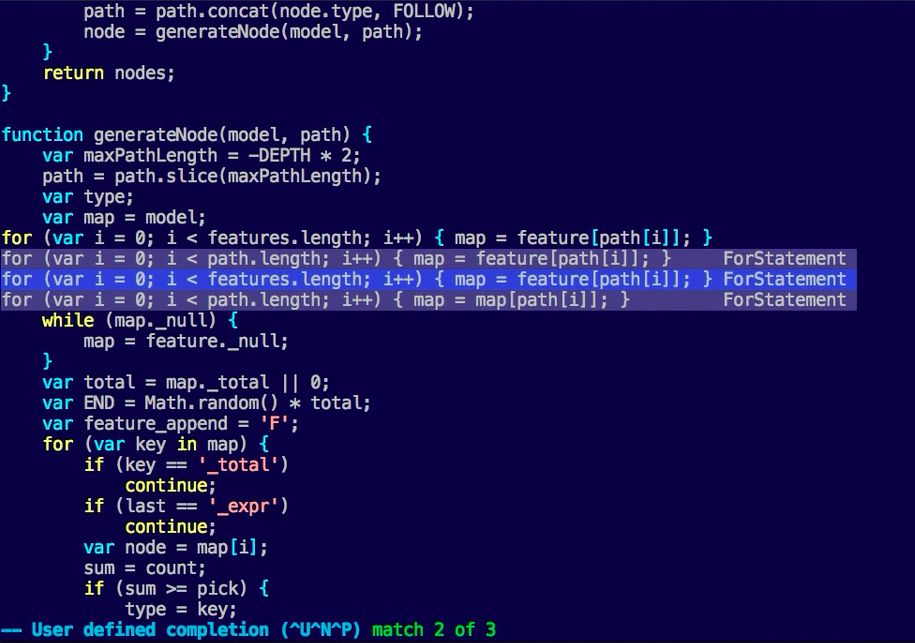
\includegraphics[width=1.00\textwidth]{vim1}
			\caption{Inserting a {\tt for} loop} \label{fig:vim1}
		\end{subfigure}
		\begin{subfigure}[h]{6cm}
			\centering
			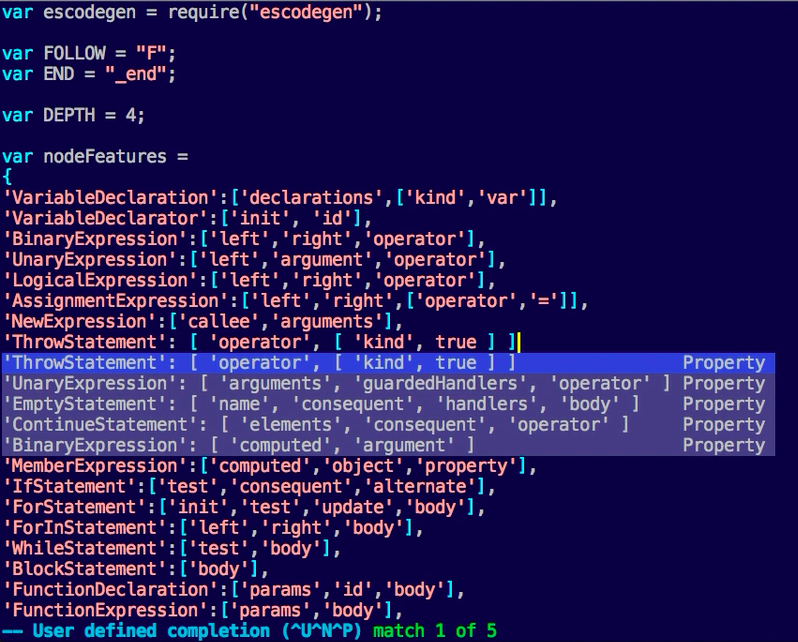
\includegraphics[width=1.00\textwidth]{vim2}
			\caption{Inserting an object property} \label{fig:vim2}
		\end{subfigure}
	\end{tabular}
	\caption{Screenshots of vim using autocomplete of programs}
\end{figure}

The vim autocomplete feature is limited to inserting program snippets on a single
line, and requires the user to explicitly trigger the \texttt{completefunc}
feature to be prompted with code snippets. To further explore using our model
for editing, we created a web-based editor that more deeply integrates Probabilistic
Programming.

\subsection{Guided IDE}

The Guided IDE offers users an environment for building a program entirely using
our model, using program snippets generated at the cursor's context as building
blocks. The editor presents a window for the program text, and a list of
suggestion code snippets. The user can move a cursor through the code window at
positions corresponding to boundaries of program nodes. As the user moves the
cursor, the snippet suggestions are regenerated using the cursor's node path, to
continuously provide suggestions relevant to the current context of the program. When the
user selects a suggestion snippet, its AST is inserted into the program's AST at
the cursor's position in the tree, and the code window is redrawn. The user can
move the cursor within newly inserted blocks, so that the program can grow
deeper. The initial corpus for the IDE's model consists of the JavaScript files
that comprise our project.

\begin{figure}[h]
  \centering
  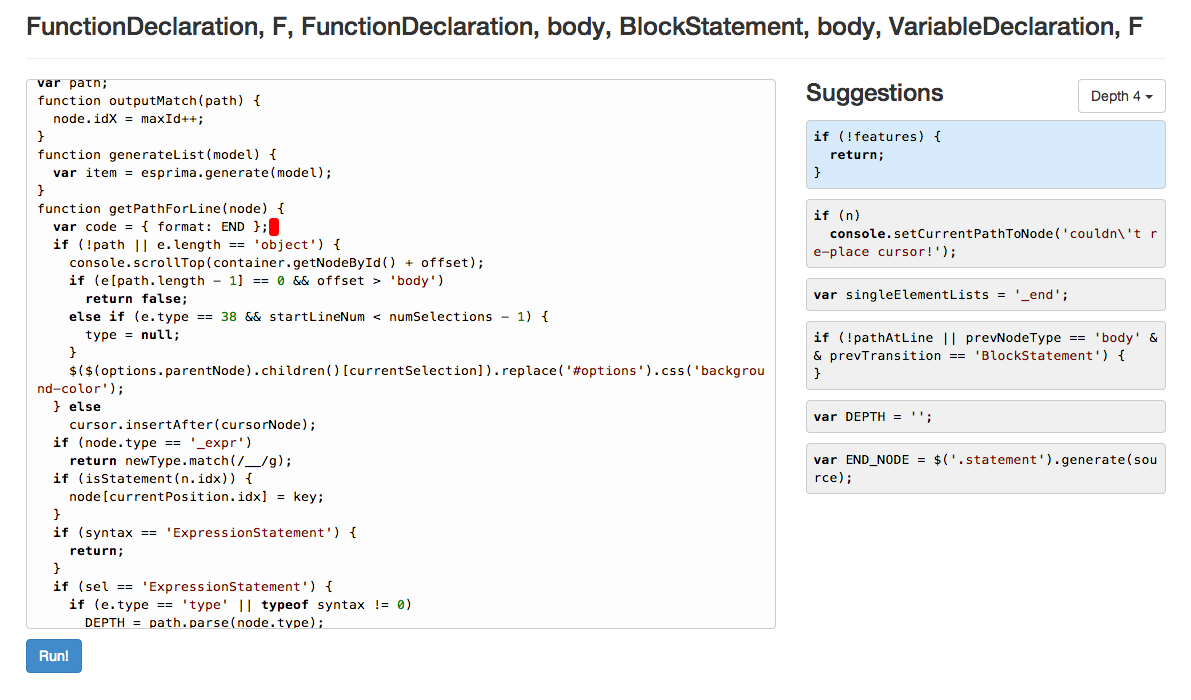
\includegraphics[width=1.00\textwidth]{ide}
  \caption{Screenshot of the web program editor GUI. The header along the top indicates the path (trimmed to the selected depth) to the current position of the cursor. Code snippets on the left can be navigated using the arrow keys.} \label{fig:screenshot}
\end{figure}

\section{Results}

\subsection{Using the IDE}

We can use the Guided IDE to generate programs. The programs look like actual
programs but do not actually function unless the user is very careful about
which snippets they pick. Crucially, the variable and identifier names that our
system generates are not in general meaningful in the scope of the generated
program.  Whereas with the vim autocompletions the identifiers would often be
valid because because the corpus was the current file, with the larger corpus of
the Guided IDE and writing a program from scratch, the user is less likely to
find program snippets that use valid identifiers.

\subsection{Limitations of the model}

It is a limitation of the current model that identifier names are chosen
probabilistically based on their position in the code, without regard to whether
they are in scope and without refering to anything in another part of the
program. Because of this limitation, the Guided IDE is not useful for practical
purposes. We consider some alternative approaches for the Guided IDE using a
similar model.

\subsection{Alternative approaches for the IDE}

\subsubsection{Prompt for identifiers}

Rather than picking identifier names from the model, use placeholder identifiers
and prompt the user to enter actual identifiers, with suggestions based on the
current variables in scope and previously used identifiers. This would give the
user the opportunity to create semantically valid programs, but the entering of
identifier names could be tedious.

\subsubsection{Stubs}

Instead of having a movable cursor in the code window, consider stubs in the
program. Each stub would be a marker in place of an AST node. The user would
select a stub and be given choices of snippets to replace it. Selecting a
snippet would move the current snippet into the program in place of the selected
stub.  The generated snippets could themselves have stubs in them, so that the
user may continue to complete stubs and expand their program.  At the level of
variable identifiers, the snippet suggestions would be taken from the computed
list of in-scope variables at the position of the selected stub, unless the
completion was for a variable declaration, in which case the user would be
prompted to name a new variable.

This approach, while offering less places to insert code then the current
approach, would allow for programs to more closely be generated from our model,
since the stub completions would always be at leaf nodes of the AST, whereas in
the current approach the user may choose to insert a snippet in the middle of a
list, which means that the transition from the inserted snippet to the following
node in the list does not in general follow from the model.

While the stub approach would be more restrictive for the user as it requires
them to build the program in a certain way, with proper handling of identifiers,
it may provide for an interesting or useful paradigm for interacting with a program
source.

\subsection{Intelligent handling of identifiers and literals}

We explored other approaches to solve the issue of generating meaningful identifiers and literals described before.

\subsubsection{Secondary models}

When generating identifiers, we were interested in generating meaningful ones rather than random ones (whose weights were calculated from counts originating from identifiers that could be in entirely different places of the program.) We wanted to design a model that could keep track of when the same variables were used in the same (or similar) place.

One idea was to, during the parse, keep track of the path at which each variable identifier was used, grouped by the identifier name. When an identifier needs to be generated, we can find that path in our secondary model, and if so, bind to a random (but weighted) identifier that has been used at that path, with the weight being based on the frequency of that identifier appearing at that path. For subsequent statements that need identifiers, the same process could occur, and, if the same variable group was chosen, it could generate the variable name that was bound to the first statement.

Another idea also involved constructing a secondary model during the parse, that kept track of statements that used the same identifier. When such statements are found, it would compute the path between those statements and increment a counter associated that path. This would represent the likelihood of two nodes connected by that path using the same identifier. Then, during code generation, whenever an identifier is needed, the generator would make a list of all variables in scope at that point, and compute the path from the variable declaration (and/or last use) to the node being generated. It would look up each path in the secondary model and assign each of the in-scope variables a weight. A variable could then be chosen based on this probability.

We suspect that this may affect the complexity of our algorithms significantly. If what the system is doing now is analogous to the behavior of a context-free grammar (i.e. by recursively generating nodes), then detection of use of the same identifiers across nodes would involve pattern-matching and perhaps even analogy-solving. This could analogously be considered more like the action of a Turing machine, which would mean that the complexity of the process could be unbounded.

Unfortunately, we were unable to implement these ideas or explore them further due to time constraints.

\subsubsection{Using a higher-order model}

Just as our approach of modeling a program with a tree-based Markov chain is a
higher order model than a linear Markov chain of the program source code tokens,
there may be applications of probabilistic modeling to higher-order
representations of programs than the AST, such as a \emph{higher-order abstract syntax}, which promises to ``incorporate name binding information in a uniform and language generic way'' \cite{hosa}. Such an application may model the relationship between different
parts of an AST, and handle scoping of variables to model identifiers
abstractly.

With a more sophisticated model of identifiers that could generate programs with
identifiers in meaningful relation to each other, Probabilistic Programming could
be used to generate semantically valid programs, for greater assistive,
expressive, and programmatic power.

\section{Conclusion}

We consider the web IDE a strong proof of concept for context-based code snippet generation. We are aware of some of its serious structural limitations, but we are confident that related concepts, such as genetic algorithms, might be possible. Specifically, we are interested in the possibility of creating genetic algorithms that take advantage of this platform to build and ``evolve'' code in a similar process. Perhaps it could even be given a purpose; for instance, to satisfy a set of given test cases.

%Other applications of the model: genetic algorithms

\subsection*{Source code \& demo}

The source code for Probabilistic Programming is available online under an open
source license:
\url{https://github.com/RocHack/jschain}.\\

\noindent The web IDE can be found at
\url{https://csug.rochester.edu/u/clehner/jschain/web/}.

\clearpage

\begin{thebibliography}{1}

	\bibitem{esprima} Ariya Hidayat {\em Esprima}
		\\\url{http://esprima.org/}

	\bibitem{markov} Takis Konstantopoulos {\em Introductory lecture notes on
		Markov Chains and Random Walks.} Uppsala University,
		\\\url{http://www2.math.uu.se/~takis/L/McRw/mcrw.pdf}

	\bibitem{hosa} Frank Pfenning, Conal Elliott
		{\em Higher-Order Abstract Syntax.}
		ACM SIGPLAN Notices. Vol. 23. No. 7. ACM, 1988.
		\\\url{http://www.cs.cmu.edu/~fp/papers/pldi88.pdf}

	\bibitem{escodegen} Yusuke Suzuki {\em Escodegen}
		\\\url{https://github.com/Constellation/escodegen}

	\bibitem{parser api} Mozilla Developer Network {\em SpiderMonkey Parser API}
		\\\url{https://developer.mozilla.org/en-US/docs/SpiderMonkey/Parser_API}

\end{thebibliography}

\clearpage
\section*{Appendix}

\begin{figure}[h!]
	\caption{JSON AST sample}
	\label{fig:sample-ast}
	\centering
    \vspace{-7pt}
	An AST generated from the program ``{\tt var x = 34;}"

	\lstinputlisting{ast-sample.json}
\end{figure}

\begin{figure}[h!]
	\caption{JSON Markov model sample}
	\label{fig:sample-model}
	\centering
    \vspace{-7pt}
	A Markov chain model generated from the program ``{\tt var x = 34;}"

	\lstinputlisting{model-sample.json}
\end{figure}

\end{document}
